\section{深度学习简介与反向传播算法}
\subsection{深度学习的历史}
\begin{description}
	\item[1958:] 感知机线性模型,感知机模型由两层构成,能够实现与或非运算.
	\item[1969:] 感知机模型存在局限,不能处理非线性可分问题.
	\item[1980:] 多层感知机模型,和现在的 DNN 模型在结构上没有太大区别.
	\item[1986:] 反向传播,解决了权重的更新问题,其实质就是梯度下降.超过三层隐藏层没有太多提高.
	\item[1989:] 低潮期,1个隐藏层已经足够好,为什么要使用深度模型,期间 svm 等方法发展迅猛.
	\item[2006:] RBM 使用受限波兹曼机对网络权重进行初始化,重新引起关注.
	\item[2009:] GPU 加速计算.
	\item[2011:]在语音识别领域开始流行.
	\item[2012:] 图像识别领域开始流行.
\end{description}

\subsection{三步骤看深度学习}

\begin{description}
	\item[选择函数模型] 选择一种深度模型架构,就是定义了一个函数集合。所以在深度学习中关键的一步不是设计何种复杂度的模型,而是设计网络结构。
	\item[评价函数优劣] 函数优劣通过损失函数衡量。损失函数为所有训练样本与目标的交叉熵。
	\item[函数寻优权重更新] 反向传播更新模型权重。
\end{description}

\section{反向传播算法}
反向传播算法的实质就是梯度下降法,对于复杂的网络模型,通过链条法则计算梯度,以便于梯度跟新。

\begin{myquotation}{链条法则}
\begin{description}
	\item[case1:] $y=f(x) \quad z=f(y)$\\
					$\Delta x \rightarrow \Delta y \rightarrow \Delta z \qquad \frac{dz}{dx}=\frac{dz}{dy} \frac{dy}{dx}$
	\item[case2:] $x=g(s) \quad y=f(s) \quad z=h(x,y)$\\
					$\frac{dz}{ds}=\frac{dz}{dx}\frac{dx}{ds} + \frac{dz}{dy}\frac{dy}{ds}$
\end{description}	
\end{myquotation}
深度网络的损失函数表示为:
\[
L(\theta) = \sum_{ n } C^{n}(\theta)
\]
为所有训练样本的损失之和,计算梯度也为所有样本的梯度之和,以某一个样本对某一权重的提示计算为例,如图所示\ref{fig:backpropagation}:
\begin{figure}[htb]
	\centering
	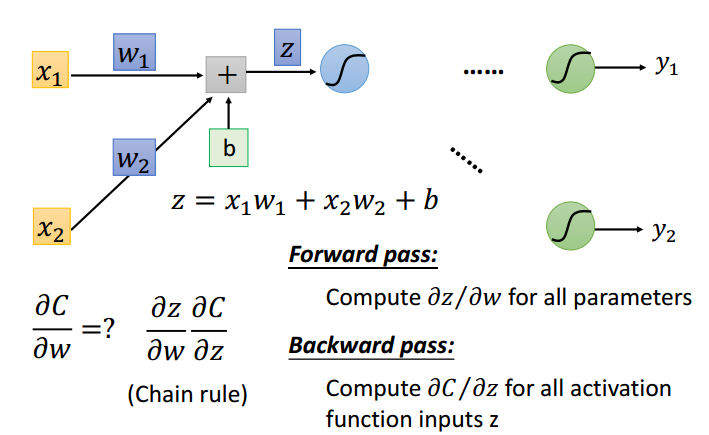
\includegraphics[scale=0.4]{pic/backpropagation}
	\caption{反向传播算法的前传过程和后传过程}
	\label{fig:backpropagation}
\end{figure}
\[
\frac{\partial C}{\partial w} = \frac{\partial C}{\partial z} \frac{\partial z}{\partial w}
\]
其中,前传过程为$\frac{\partial z}{\partial w}=x$,后传过程为$\frac{\partial C}{\partial z}$.
计算前传过程的值为前向传播时权重乘的值()神经元的输出值),后传过程$$\frac{\partial C}{\partial z}$$从两种情况加以考虑:

\begin{description}
 \item[后接输出层] 直接链式计算导数
\item[其它隐层] 递归计算
\end{description}

详细计算过程见图\ref{fig:backwardpass}:
\begin{figure}[htb]
	\centering
	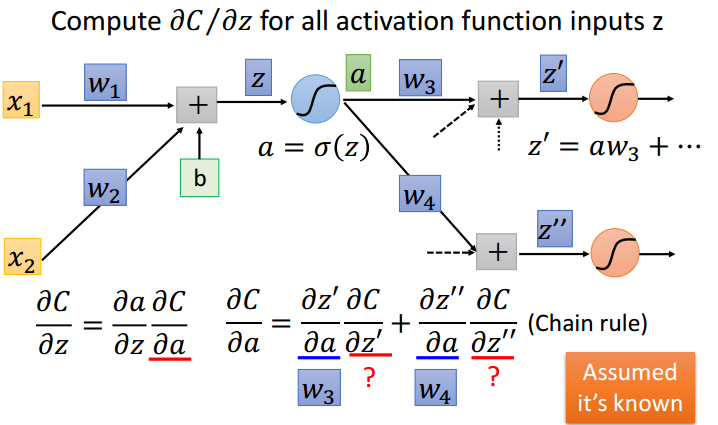
\includegraphics[scale=0.4]{pic/backwardpass_01}
	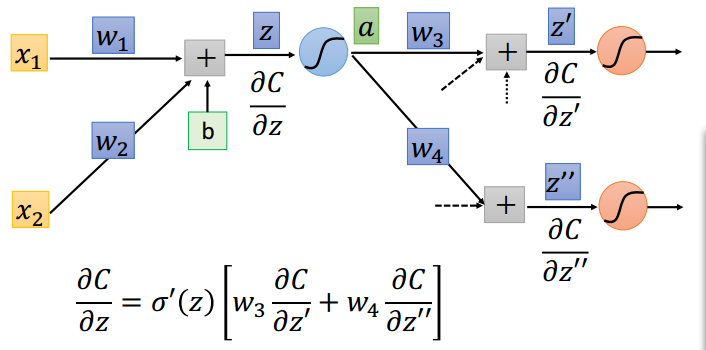
\includegraphics[scale=0.4]{pic/backwardpass_02}
	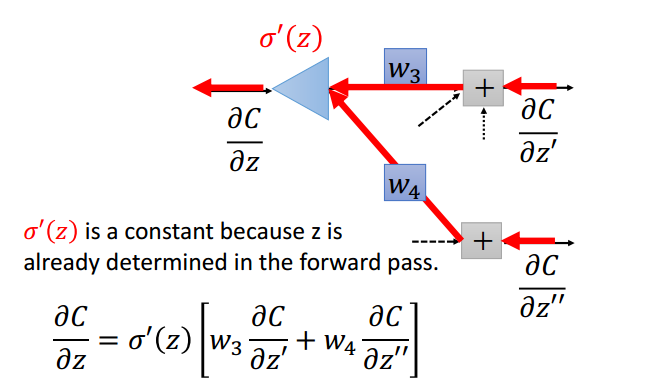
\includegraphics[scale=0.4]{pic/backwardpass_03}
	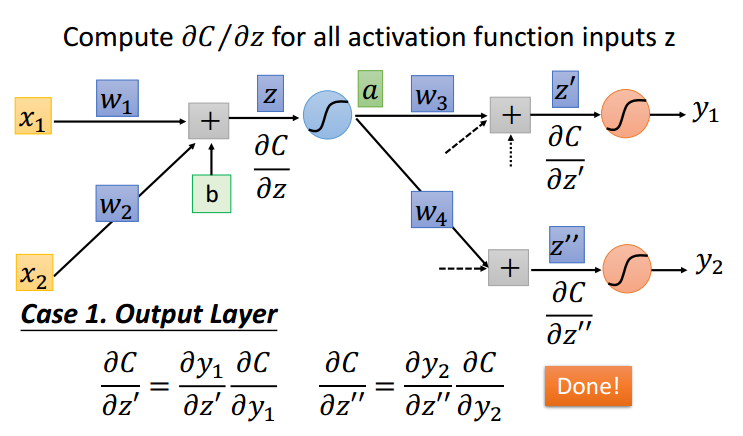
\includegraphics[scale=0.4]{pic/backwardpass_04}
	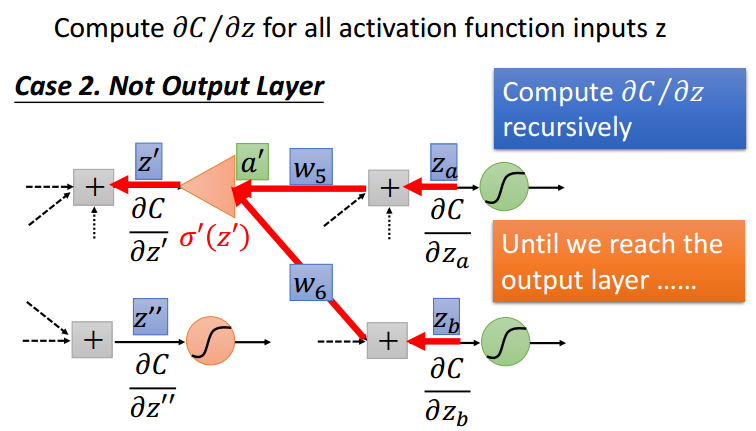
\includegraphics[scale=0.4]{pic/backwardpass_05}
	\caption{后传过程计算}
	\label{fig:backwardpass}
\end{figure}
\clearpage